\documentclass{article}
\usepackage{amsmath}
\usepackage{amssymb}
\usepackage{graphicx}
\usepackage{hyperref}
\usepackage[version=4]{mhchem}


\begin{document}
As shown in the figure, \(\triangle A B C\) is a right triangle with \(\angle C=90^{\circ} . A C\) is the diameter of circle \(O\). Circle \(O\) meets the hypotenuse \(A B\) at \(D\). Draw the tangent through \(D\) to the circle to meet the leg \(B C\) at \(E\). Prove: \(B E=E C\).

Solution:
\begin{center}
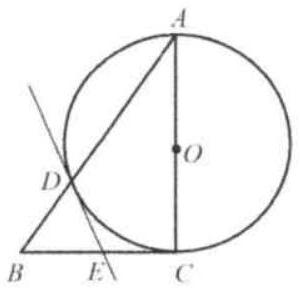
\includegraphics[width=\textwidth]{images/194(3).jpg}
\end{center}


Connect CD, EO.\\
Since \(A C\) is the diameter, \(\angle A D C=90^{\circ}\). We also know that \(\angle A C B=90^{\circ}\)\\
Let \(\angle A=\alpha, \angle B=\angle A C D=\beta\).\\
Then \(\angle O D C=\angle O C D=\beta\)\\
We also have \(\angle O D C=\angle O E C=\beta\) (they all face the same arc \(O C\) ).\\
Thus \(\angle A B C=\angle O E C=\beta\) and \(A B / / O E\).\\
Since \(O\) is the midpoint of \(A C, E\) must be the\\
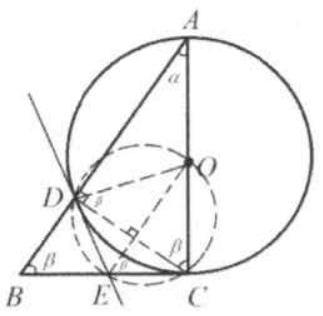
\includegraphics[width=\textwidth]{images/195(2).jpg} midpoint of \(B C\).\\
That is, \(B E=E C\).


\end{document}
